\documentclass[aspectratio=169]{beamer}

\usepackage[brazil]{babel}
\usepackage[utf8]{inputenc}
\usepackage[T1]{fontenc}

\usetheme{Madrid}

\setbeamertemplate{navigation symbols}{}

\title[Gestão Organizacional]{Gestão Organizacional}

\author[Diego S. C. Nascimento]{Diego Silveira Costa Nascimento}

\institute[IFRN]{
	Instituto Federal de Educação, Ciência e Tecnologia do Rio Grande do Norte\\
	Campus Natal -- Cidade Alta\\
	diego.nascimento@ifrn.edu.br
}

\date[\today]{\today}

\begin{document}

\begin{frame}[plain]
	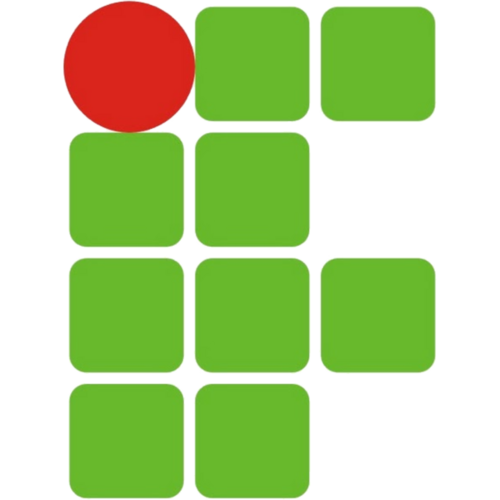
\includegraphics[scale=0.2]{img/IFRN}
	\titlepage
\end{frame}

\logo{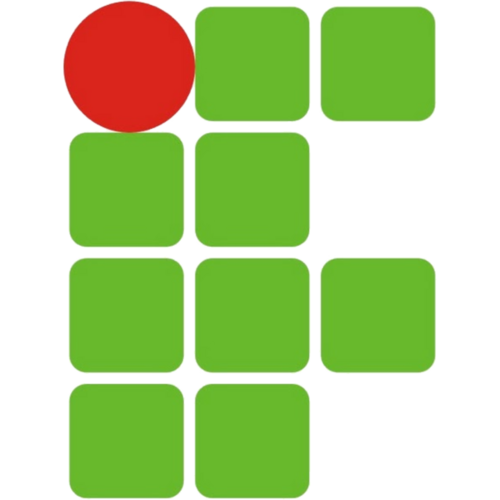
\includegraphics[scale=0.1]{img/IFRN}}

\AtBeginSection[]{
	\begin{frame}
		\frametitle{Sumário}
		\tableofcontents[currentsection]
	\end{frame}
}

\section{Teoria Geral da Administra\c cão}

\begin{frame}
	\frametitle{O que é Teoria Geral da Administra\c cão (TGA)?}

	\begin{block}{Defini\c cão}
	É o conjunto de conhecimentos a respeito das organiza\c cões e do processo de administrá-las, sendo composta por princípios, proposi\c cões e técnicas em permanente elabora\c cões.
	\end{block}
\end{frame}

\begin{frame}
	\frametitle{História}

	\begin{itemize}
		\item A administra\c cão surgiu na Suméria a 5.000 A.C.;
		\item Os habitantes procuravam uma maneira para melhorar a resolu\c cão dos seus problemas;
		\item Logo surge a arte e o exercício de administrar.
	\end{itemize}
\end{frame}

\begin{frame}
	\frametitle{Frederick Taylor}

	\begin{itemize}
		\item É considerado o pai da administra\c cão científica;
		\item Nascido nos Estados Unidos;
		\item Para determinar a melhor forma de executar um trabalho, dividiu cada atividades em movimentos menores e cronometrou cada um deles;
		\item Analisou a a\c cão para eliminar movimentos desnecessários, o que dava a origem ao método mais ágil e eficiente de executar uma tarefa atribuída;
		\item Traz os conceitos de eficiência e eficácia no meio da produ\c cão industrial.
	\end{itemize}
\end{frame}

\begin{frame}
	\frametitle{Eficiência vs Eficácia}

\begin{columns}
	\column{0.5\textwidth}
		
	\begin{itemize}
		\item Fazer bem as coisas;
		\item Preocupa\c cão com os meios;
		\item Ênfase no processo; e
		\item Ausência de desperdícios.
	\end{itemize}

	\column{0.5\textwidth}

	\begin{itemize}
		\item Fazer as coisas certas;
		\item Preocupa\c cão com os fins;
		\item Ênfase nos resultados; e
		\item Maximizar os objetivos.
	\end{itemize}
\end{columns}

\end{frame}

\begin{frame}
	\frametitle{Teoria Científica de Taylor}

	\begin{itemize}
		\item Mecanicismo;
		\item Superespecializa\c cão do trabalhador;
		\item Visão microscópica do homem;
		\item Abordagem de sistema fechado; e
		\item A explora\c cão dos empregados.
	\end{itemize}
\end{frame}

\begin{frame}
	\frametitle{Henry Ford}

	\begin{itemize}
		\item Foi um empresário norte-americano;
		\item Fundador da Ford Motor Company;
		\item O primeiro a implantar uma linha de montagem em série na fabrica\c cão de automóveis.
	\end{itemize}
\end{frame}

\begin{frame}
	\frametitle{Princípios de Ford }

	\begin{itemize}
		\item Princípio da intensifica\c cão;
		\item Princípio da economicidade; e
		\item Princípio da produtividade.
	\end{itemize}
\end{frame}

\begin{frame}
	\frametitle{Henri Fayol}

	\begin{itemize}
		\item Nascido na Fran\c ca;
		\item Foi fundador da teoria clássica da administra\c cão;
		\item Foi o primeiro a tratar a administra\c cão como disciplina para formar lidenra\c cas qualificadas;
		\item Toma como base a busca por máxima eficiência através da visão homem econônico;
		\item Ou seja, considera o homem como racional e com focos racionais;
		\item Criou um sistema para otimizar a gerência dando a cada gerente o seus deveres.
	\end{itemize}
\end{frame}

\begin{frame}
	\frametitle{Fun\c cões Administrativas de Fayol}

	\begin{itemize}
		\item Planejar;
		\item Organiza\c cão;
		\item Dire\c cão; e
		\item Controle.
	\end{itemize}
\end{frame}

\begin{frame}
	\frametitle{Max Weber}

	\begin{itemize}
		\item Nascido na Alemanha; e
		\item Fundou o método de análise sociológica.
	\end{itemize}
\end{frame}

\begin{frame}
	\frametitle{Princípios de Max Weber}

	\begin{itemize}
		\item Indivíduo;
		\item Ética; e
		\item Rela\c cão social.
	\end{itemize}
\end{frame}

\end{document}